%
% Copyright (C) 2004-2009 Jason Blevins <jrblevin@sdf.lonestar.org>
% http://jblevins.org/projects/cv-template/
%
% You may use use this document as a template to create your own CV
% and you may redistribute the source code freely. No attribution is
% required in any resulting documents. I do ask that you please leave
% this notice and the above URL in the source code if you choose to
% redistribute this file.

\documentclass[letterpaper, 10pt]{article}

\usepackage{hyperref}
\usepackage{geometry}

%%%%%%%%%%%%%%%%%%%%%%%%%%%%%%%%%%%%%%%%%%%%%%%%%%%%%%%%%%%%%%%%%%%%%%%%%%%%%%%%%
\usepackage[minbibnames=3,sorting=ndymdt,date=comp,isbn=false,doi=false,defernumbers=true,backend=biber]{biblatex}

% https://tex.stackexchange.com/a/408041
\NewBibliographyString{toappear}
\DefineBibliographyStrings{english}{%
  toappear = {to appear},
}

\renewbibmacro*{in:}{%
  \iffieldundef{pubstate}
    {}
    {\printfield{pubstate}%
     \setunit{\addspace}%
     \clearfield{pubstate}}%
  \printtext{%
    \bibstring{in}\intitlepunct}}

\addbibresource[]{papers.bib}
\addbibresource[]{presentations-conference.bib}
\addbibresource[]{presentations-invited.bib}
\addbibresource[]{presentations-other.bib}

\DeclareSortingTemplate{ndymdt}{
	\sort[direction=descending]{
		\field{sortyear}
		\field{year}
		\literal{9999}
	}
	\sort[direction=descending]{
		\field[padside=left,padwidth=2,padchar=0]{month}
		\literal{99}
	}
	\sort[direction=descending]{
		\field[padside=left,padwidth=2,padchar=0]{day}
		\literal{99}
	}
	\sort{
		\field{presort}
	}
	\sort[final]{
		\field{sortkey}
	}
	\sort{
		\field{sortname}
		\field{author}
		\field{editor}
		\field{translator}
		\field{sorttitle}
		\field{title}
	}
	\sort{
		\field{sorttitle}
	}
	\sort[direction=descending]{
		\field[padside=left,padwidth=4,padchar=0]{volume}
		\literal{9999}
	}
}

\usepackage{graphicx}



%\usepackage[sfdefault]{cabin}
%\usepackage[T1]{fontenc}

%\usepackage[sfdefault]{overlock} %% Option 'sfdefault' only if the base font of the document is to be sans serif
\usepackage[default,oldstyle,scale=0.95]{opensans}

\usepackage[T1]{fontenc}

\usepackage{enumitem}
\usepackage{setspace}
	\onehalfspacing
\usepackage{xcolor}

% Set your name here
\def\name{George G. Vega Yon, Ph.D.}

% Replace this with a link to your CV if you like, or set it empty
% (as in \def\footerlink{}) to remove the link in the footer:
\def\footerlink{https://ggvy.cl}

% The following metadata will show up in the PDF properties
\hypersetup{
  colorlinks = true,
  urlcolor = teal,
  pdfauthor = {\name},
  pdfkeywords = {statistics, mathematics, statistical computing, data science, machine learning},
  pdftitle = {\name: Curriculum Vitae},
  pdfsubject = {Curriculum Vitae},
  pdfpagemode = UseNone
}

\geometry{
%  body={6.5in, 9in},
% margin=.8in
  left=1in,
  top=1in,
  right=1in,
  bottom=1in
}

% Customize page headers
\usepackage{fancyhdr}
%\pagestyle{myheadings}
%\markright{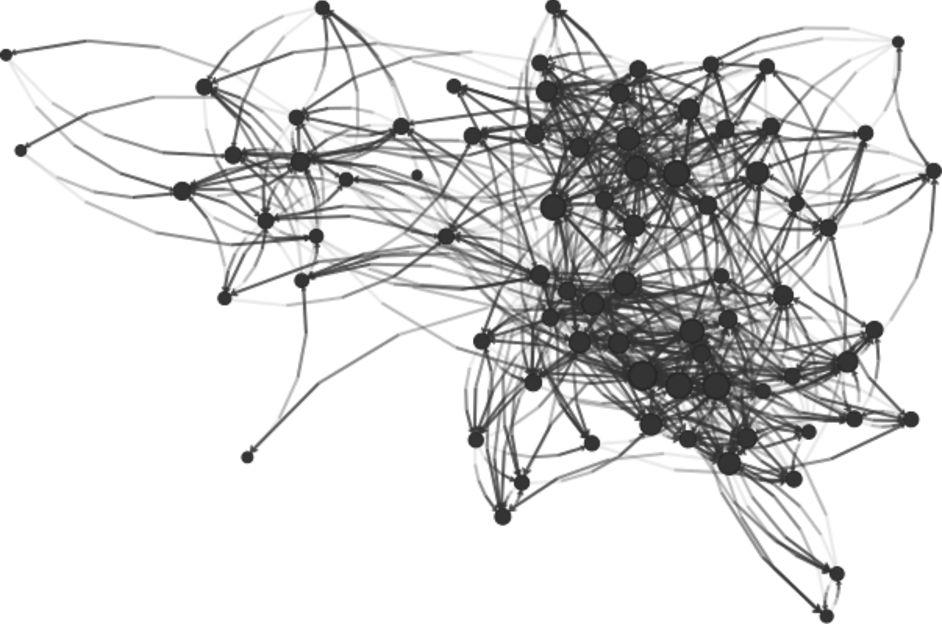
\includegraphics[width=1cm]{fig/ukfaculty.pdf} \name}
\pagestyle{fancy}
\fancyhead{}
\fancyfoot{}
\renewcommand{\headrulewidth}{0pt}
\fancyhead[L]{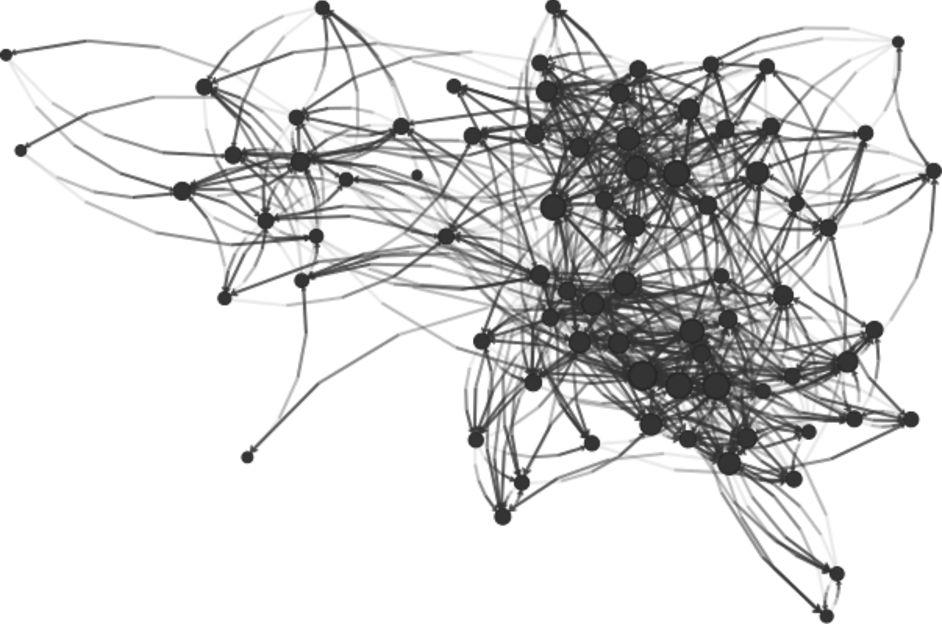
\includegraphics[width=1cm]{fig/ukfaculty.pdf}\\\vspace{-.75cm}\hspace{1.1cm}\emph{\name}}
\fancyhead[R]{\small\thepage}
\thispagestyle{empty}

% Para poder poner comandos genericos en tablas (en el inicio del argumento)
\usepackage{array}

\renewcommand{\bf}{\bfseries\color{teal}}
\renewcommand{\textbf}[1]{{\bfseries\color{teal}#1}}

\begin{document}

% Place name at left
\hfill 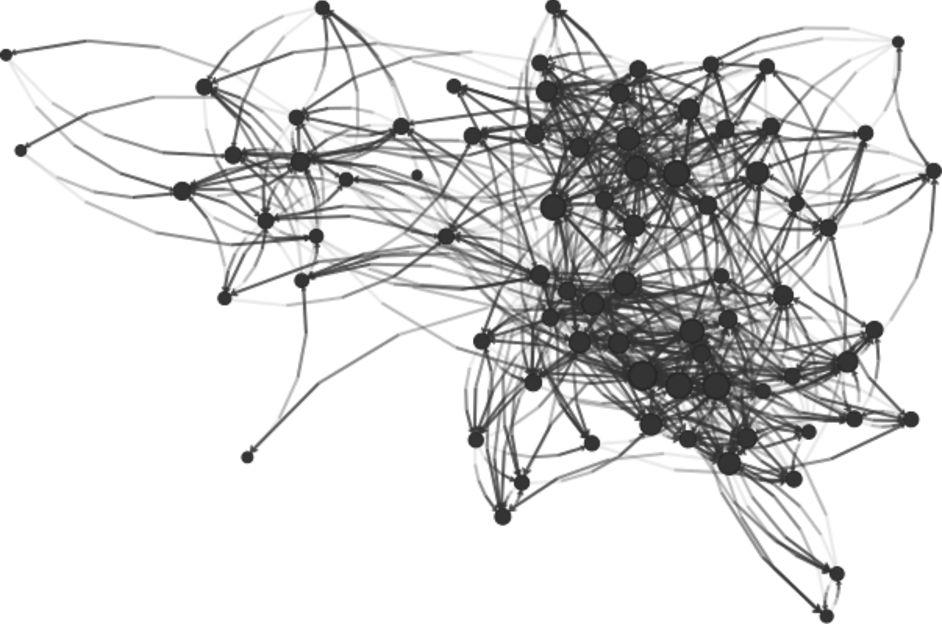
\includegraphics[width=.4\linewidth]{fig/ukfaculty.pdf}\vspace{-6cm}
\part*{\color{darkgray}{\name}}


\begin{minipage}{0.50\linewidth}
  \begin{tabular}{>{}p{.2\linewidth}p{.79\linewidth}}
    Mobile & +1 (six two six) 381 8171 \\
    e-mail & \href{mailto:g.vegayon@gmail.com}{\tt g.vegayon@gmail.com} \\
    website & \href{https://ggvy.cl}{\tt ggvy.cl} \\
    Code & \href{https://github.com/gvegayon}{\tt github.com/gvegayon}\\
    Linkedin & \href{https://www.linkedin.com/in/georgevegayon/}{\tt www.linkedin.com/in/georgevegayon/} \\
    ORCID & \href{https://orcid.org/0000-0002-3171-0844}{\tt orcid.org/0000-0002-3171-0844}
  \end{tabular}
\end{minipage}


\section*{Education}

%\begin{itemize}

\noindent 
{\bf Ph.D. in Biostatistics (with a concentration in Statistical Computing)}\hfill 2020\\
University of Southern California, USA.\\
Dissertation title:\\ \hspace*{.5cm}\emph{``Essays on Bioinformatics and Social Network Analysis:\\\hspace*{.75cm}Statistical and Computational Methods for Complex Systems.''}\vspace{.5cm}

\noindent {\bf M.Sc. in Social Sciences (with a concentration in Economics)}\hfill 2016\\
California Institute of Technology, USA.\vspace{.5cm}

\noindent {\bf Master in Economics and Public Policy}\hfill 2011\\Universidad Adolfo Ib\'a\~nez, Chile. \vspace{.5cm}

\noindent {\bf BS. in Business Administration} (with a minor in Political Science) \hfill 2011\\Universidad Adolfo Ib\'a\~nez, Chile.
%\end{itemize}

\section*{Awards}

\noindent Top paper award, International Communication Association\hfill 2022 

\noindent Travel Grant, Society of Young Network Scientist\hfill 2019%\vspace{.5cm}

\noindent Fellowship, California Institute of Technology\hfill 2014%\vspace{.5cm}

\noindent Honorable Mention (Posters Session) Chilean Economics Society\hfill 2012%\vspace{.5cm}

\noindent Scholarship, Universidad Adolfo Ib\'a\~nez\hfill 2006

\section*{Major Areas of Research Interest}

Social Networks and Complex Systems\\
Statistical Computing\\
Scientific Software Development \\
Mechanistic Machine Learning\\
Statistical Methods Development

\section*{Academic and Professional Experience} 

%\begin{itemize}
\noindent \textbf{Lead Data Scientist (Associate)}\hfill Nov 2023 -- Present\\Booz Allen Hamilton\vspace{.5cm}

\noindent \textbf{Research Assistant Professor}\hfill Nov 2021 -- Present\\Division of Epidemiology, University of Utah\vspace{.5cm}

\noindent \textbf{Adjunct Assistant Professor}\hfill Jan 2023 -- Present\\Division of Population Health Sciences, University of Utah\vspace{.5cm}

\noindent \textbf{Research Programmer}\hfill Feb 2018 -- Nov 2021\\{Department of Preventive Medicine, University of Southern California}\vspace{.5cm}

\noindent \textbf{Programmer Analyst}\hfill Oct 2015 -- Feb 2018\\Department of Preventive Medicine, University of Southern California.\vspace{.5cm}

\noindent \textbf{Graduate student researcher}\hfill Aug 2011 -- Oct 2015\\Division of Social Sciences, California Institute of Technology.\vspace{.5cm}

\noindent \textbf{Analyst}\hfill Aug 2011 -- Aug 2014\\
Research Division, Chilean Pension Supervisor (Pension System Watchdog).\vspace{.5cm}

\noindent \textbf{Founding partner}\hfill Jan 2012 -- Jan 2014\\
Nodos Chile Social Network Analysis Ltda.\vspace{.5cm}

\noindent \textbf{Adjunct Professor of Statistical Computing}\hfill Jan 2011 -- Jun 2012\\School of Government, Universidad Adolfo Ib\'a\~nez. 


\section*{Peer Reviewed Publications}
\nocite{*}

\printbibliography[title=\vskip-20pt,keyword=published,resetnumbers=true]

\section*{Work in Progress and Technical Reports}

\printbibliography[title=\vskip-20pt,keyword=wip,resetnumbers=1]

\section*{Books}

\noindent ``Applied Network Science with R'' (on development) \url{https://book.ggv.cl/}

\noindent ``Applied HPC with R'' (on development) \url{https://book-hpc.ggv.cl/}


\section*{Software Packages}

\begin{enumerate}[label={[}\arabic*{]},labelindent=5\parindent,labelsep=8pt]
\item \textbf{George G.} \textbf{Vega Yon}. \textit{defm: Estimation and simulation of Multi-binary response models} (2023). R package version 0.1.0. {\small URL}: \url{htps://cran.r-project.org/package=defm}. \\
\includegraphics[width=2.5cm]{fig/cran-downloads-defm.pdf} 
\item Derek Meyer, \textbf{George G.} \textbf{Vega Yon}. \textit{epiworldR: Fast Agent-Based Epi Models} (2023). R package version 0.0-2. {\small URL}: \url{https://cran.r-project.org/package=epiworldR}. \\
\includegraphics[width=2.5cm]{fig/cran-downloads-epiworldr.pdf} 
\item \textbf{George G.} \textbf{Vega Yon}. \textit{aphylo: Statistical Inference of Annotated Phylogenetic Trees} (2022). R package version 0.2-1. {\small URL}: \url{https://cran.r-project.org/package=aphylo}. \\
\includegraphics[width=2.5cm]{fig/cran-downloads-aphylo.pdf} 
\item \textbf{George G.} \textbf{Vega Yon}. \textit{A Flexible and General Agent Based Model Engine} (2022). C++ library version 0.0-1. {\small URL}: \url{https://github.com/UofUEpiBio/epiworld}.  
\item \textbf{George G.} \textbf{Vega Yon}. \textit{netplot: Beautiful graph drawing} (2021). R package version 0.1-1. {\small URL}: \url{https://cran.r-project.org/package=netplot}. \\
\includegraphics[width=2.5cm]{fig/cran-downloads-netplot.pdf} 
\item \textbf{George G.} \textbf{Vega Yon}. \textit{rgexf: Build, Import and Export GEXF Graph Files} (2020). R package version 0.16.0. {\small URL}: \url{https://CRAN.R-project.org/package=rgexf}. \\
\includegraphics[width=2.5cm]{fig/cran-downloads-rgexf.pdf} 
\item \textbf{George G.} \textbf{Vega Yon}, Thomas Valente. \textit{{{netdiffuseR: Analysis of Diffusion and Contagion Processes on Networks}}} (2020). R package version 1.22.0. {\small URL}: \url{https://github.com/USCCANA/netdiffuseR}. \\
\includegraphics[width=2.5cm]{fig/cran-downloads-netdiffuser.pdf} 
\item \textbf{George G.} \textbf{Vega Yon}, Kayla de la Haye. \textit{ergmito: Exponential Random Graph Models for Small Networks} (2020). R package version 0.3-0. {\small URL}: \url{https://cran.r-project.org/package=ergmito}. \\
\includegraphics[width=2.5cm]{fig/cran-downloads-ergmito.pdf} 
\item \textbf{George G.} \textbf{Vega Yon}. \textit{slurmR: A Lightweight Wrapper for 'Slurm'} (2020). R package version 0.4-1. {\small URL}: \url{https://CRAN.R-project.org/package=slurmR}. \\
\includegraphics[width=2.5cm]{fig/cran-downloads-slurmr.pdf} 
\item \textbf{George G.} \textbf{Vega Yon}. \textit{fmcmc: A friendly MCMC framework} (2020). R package version 0.3-0. {\small URL}: \url{https://CRAN.R-project.org/package=fmcmc}. \\
\includegraphics[width=2.5cm]{fig/cran-downloads-fmcmc.pdf} 
\item \textbf{George G.} \textbf{Vega Yon}. \textit{barry: your to-go motif accountant} (2020). C++ library version 0.0-1. {\small URL}: \url{https://github.com/USCbiostats/barry}.  
\item \textbf{George G.} \textbf{Vega Yon}. \textit{pruner: Implementing the Felsenstein's Tree Pruning algorithm} (2020). C++ library version 0.0-1. {\small URL}: \url{https://github.com/USCbiostats/pruner}.  
\item \textbf{George G.} \textbf{Vega Yon}, Brian Quistorff. \textit{parallel: Stata Module for Parallel Computing} (2019). Stata Module version 1.20.0. {\small URL}: \url{https://github.com/gvegayon/parallel}.  
\item \textbf{George G.} \textbf{Vega Yon}. \textit{googlePublicData: Working with Google's 'Public Data Explorer' DSPL Metadata Files} (2017). R package version 0.16.1. {\small URL}: \url{https://CRAN.R-project.org/package=googlePublicData}. \\
\includegraphics[width=2.5cm]{fig/cran-downloads-googlepublicdata.pdf} 
\item \textbf{George G.} \textbf{Vega Yon}, Enyelbert Mu~noz. \textit{ABCoptim: Implementation of Artificial Bee Colony (ABC) Optimization} (2017). R package version 0.15.0. {\small URL}: \url{https://CRAN.R-project.org/package=ABCoptim}. \\
\includegraphics[width=2.5cm]{fig/cran-downloads-abcoptim.pdf} 
\item \textbf{George G.} \textbf{Vega Yon}. \textit{{twitterreport: Out-of-the-box analysis and 
	reporting tools for twitter}} (2016). R package version 0.16. {\small URL}: \url{https://doi.org/10.5281/zenodo.44528}.  

\end{enumerate}

%\pagebreak

\section*{Conference talks/workshops}

\printbibliography[title=\vskip-20pt,keyword=conferencetalk, resetnumbers=true]

%\pagebreak

\section*{Invited Speaker}

\printbibliography[title=\vskip-20pt,keyword=invitedtalk, resetnumbers=true]

\section*{Other Talks}

\printbibliography[title=\vskip-20pt,keyword=othertalk, resetnumbers=true]

\section*{Teaching}

%\begin{itemize}
	\noindent \textbf{Statistical Inference in Network Science} \hfill Summer 2024\\
	Universidad del Desarrollo, Chile\\
	Instructor, Social Complexity Summer School\vspace{.5cm}

	\noindent \textbf{Exponential-Family Random Graph Models} \hfill Summer 2024\\
	Chilean Society for Social Network Analysis (ChiSocNet), Chile\\
	Co-Instructor, 1st Chilean Summer School about Social Network Research\vspace{.5cm}

	\noindent \textbf{(PHS 7045) Advanced Programming with R and HPC} \hfill Fall 2022\\
The University of Utah, USA\\
Co-instructor, PHS Ph.D. Program\vspace{.5cm}

\noindent \textbf{(PM 566) Introduction to Health Data Science} \hfill Fall 2021\\
	University of Southern California, USA\\
	Instructor, Masters of Science in Public Health Data Science\vspace{.5cm}

\noindent \textbf{(PM 566) Introduction to Health Data Science} \hfill Fall 2020\\
	University of Southern California, USA\\
	Co-instructor, Masters of Science in Public Health Data Science\vspace{.5cm}
	
%	\item[] \textbf{R Bootcamp For Statistical Computing (online workshop)} (Fall 2020)\\
%	University of Southern California, USA\\
%	Co-instructor and organizer, Open to members of the Keck School of Medicine
%	
%	\item[] \textbf{R Bootcamp For Statistical Computing (workshop)} (Fall 2019)\\
%	University of Southern California, USA\\
%	Co-instructor and organizer, Open to members of the Keck School of Medicine
%	
%	\item[] \textbf{R Bootcamp For Statistical Computing (workshop)} (Fall 2018)\\
%	University of Southern California, USA\\
%	Co-instructor and organizer, Open to members of the Keck School of Medicine
	

\noindent \textbf{Statistical Computing with Stata} \hfill First semester 2012\\
	Universidad Adolfo Ibáñez, Chile\\
	Instructor, Masters in Economics and Public Policy\vspace{.5cm}
	

\noindent \textbf{Introduction to Economics} \hfill First semester 2012\\
	Universidad Adolfo Ibáñez, Chile\\
	Co-instructor, B.A. in Business Administration\vspace{.5cm}
	

\noindent \textbf{Microeconomics} \hfill Second semester 2012\\
	Universidad Adolfo Ibáñez, Chile\\
	Co-instructor, B.A. in Business Administration\vspace{.5cm}
	

\noindent \textbf{Introduction to Economics} \hfill First semester 2011\\
	Universidad Adolfo Ibáñez, Chile\\
	Co-instructor, B.A. in Business Administration
% \end{itemize}

\section*{Mentoring/Advising}

\noindent \textbf{Mentor, RA (2023--Present)}\\
Hyrum Thomas Diesen, University of Utah, School of Biological Sciences, Molecular Cellular Evolutionary Biology Ph.D. program.\vspace{.5cm}

\noindent \textbf{Ph.D. Dissertation Committee Member (2023--Present),}\\ Eric Anto, University of Utah, Population Health Sciences, Biostatistics Ph.D. program.\vspace{.5cm}

\noindent \textbf{Qualifying Exam chair and Member, Ph.D. Dissertation Committee Member (2022--Present),}\\ Katherine Lawson Michod, University of Utah, Population Health Sciences, Clinical and Translational Epidemiology Ph.D. program.\vspace{.5cm}

\noindent \textbf{Mentor, RA (Summer 2023),}\\ Porter Bischoff, University of Utah + Utah Valley University, Summer Program for Undergraduate Research (SPUR), Network Visualization using R.\vspace{.5cm}

\noindent \textbf{Supervisor, RA, and M.Sc. Dissertation Committee Member (2022--Present)}\\ Derek Meyer, University of Utah, Population Health Science, Agent-Based Models for Epidemics.\vspace{.5cm}

\noindent \textbf{Mentor, (2022--Present),}\\ Jacqueline M. Kent-Marvik, University of Utah, Nursing School, Ph.D. Health Sciences, Network Science and Social Network Analysis.\vspace{.5cm}

\noindent \textbf{Mentor, (2022),}\\ Luis Lopez, NIH, Postbac program, Exponential-Family Random Graph Models.

\section*{Grants}

\noindent 5P01CA196569-08 (PIs: Gauderman, Siegmund)\hfill 07-01-2016 -- 08-31-2027\\
National Cancer Institute (NCI)\hfill 0.6 calendar months/year\\
\textbf{Statistical Methods for Integrative Genomics in Cancer}\\
This program aims to develop novel statistical methods for integrating multi-omic data to address cancer etiology, prognosis, and treatment. The program has three synergetic projects, one using evolutionary models for annotating genes and their products (of which I am a Co-I). \\
Role: Co-Investigator\\
Total Award Amount (including indirect costs): \$ 12,894,663. \vspace{.5cm}

\noindent HT94252310221 (PI: Kennedy)\hfill 07-01-2023 -- 30-06-2026\\
U.S. Army Medical Research and Development Command (DoD)\hfill 1.8 calendar months/year\\
\textbf{Phenotypes of Epilepsy Etiology and Drug Resistance (PEER)}\\
The project aims to investigate the causes and workings of epilepsy by utilizing new data science methods. The grant will be utilized to analyze patterns in three ongoing and established studies, generating "risk scores" for epilepsy after a head injury, specifically among military personnel..\\
Role: Co-Investigator\\
Total Award Amount (including indirect costs): \$ 846,484. \vspace{.5cm}

\noindent 5U01CK000675-01 (PI: Keegan)\hfill 09-30-2022 -- 09-29-2025\\
National Center for Emerging and Zoonotic Infectious Diseases (NCEZID)\hfill 0.3 calendar months/year\\
\textbf{TRANSMIT: Training Research Acumen in Students Modeling Infectious Threats}\\
A fellowship program oriented to train students in using mathematical modeling and computational methods to study infectious diseases.\\
Role: Co-Investigator\\
Total Award Amount (including indirect costs): \$ 891,356. \vspace{.5cm}

\noindent \textit{Submitted but not funded}\\

\noindent 1R01HG012878-01 (PI: Vega Yon)\hfill 12-01-2022 -- 11-30-2027\\
National Human Genome Research Institute (NHGRI)\\
\textbf{Improving our Predictive Capability of Gene Functions by Leveraging Biological Insights with Advanced Statistical Computing}\\
Using discrete exponential-family models, build a mechanistic gene function evolution model incorporating complex features involving biological processes such as neofunctionalization.\\
Role: PI\\
Total Award Amount: Not funded \vspace{.5cm}

\noindent 1R01HG012878-01A1	(PI: Vega Yon)\hfill 12-01-2023 -- 11-30-2028\\
National Human Genome Research Institute (NHGRI)\\
\textbf{Building a Novel Prediction Framework Leveraging Biological Insights to Boost Machine Learning Algorithms for Annotating Gene Function} \\
This project extends my model of function evolution using discrete exponential-family models. It embeds it into a mechanistic machine learning framework--mixing theory and data-driven models to improve gene function prediction.\\
Role: PI\\
Total Award Amount: Not funded \vspace{.5cm}



% \noindent \textbf{}
% 
% TEACHING RESPONSIBILITIES/ASSIGNMENTS
%    Mentoring/Advising
% PhD/Doctorate
% 
% 2022 - Present               Chair, Qualifying Exam and Member, Dissertation Committee, Katherine Lawson Michod, University of Utah, Population Health Sciences, Clinical and Translational Epidemiology PhD program. Title of project.

\section*{Honors and Services to the Profession}

%\begin{itemize}
%\item \textbf{Book reviewer} ``Microeconometrics and MATLAB'', by Abi Adams, Damian Clarke \& Simon Quinn, Oxford University Press, (forthcoming 2015).

\noindent\textbf{Manuscript Review (Ad Hoc)} \\
Journal of the American Statistical Association \\
American Sociological Review\\
The Official Journal of The Society for Computational Economics\\
The R Journal\\
The Stata Journal\\
Social Networks\\
Journal of Mathematical Sociology\\
Computer Methods and Programs in Biomedicine Update\\
Journal of Open Source Software\\
Bioinformatics\vspace{.5cm}

\noindent\textbf{Abstract Review} \\
International Conference on Computational Social Science (2019--2021)\\
SUNBELT Conference (2016)\vspace{.5cm}

\noindent\textbf{Panelist/Discussant}\\

\noindent ``Learning tips for your PhD from other researchers in the community''.\\ Early and Middle Career Researchers (EMCRs) on Social Networks workshops, October 2023.\\\\
``JASA A\&CS Special Invited Session: A Tale of Two Datasets -- Representativeness and Generalisability of Inference for Samples of Networks.''\\ Joint Statistical Meetings (JSM), August 2023.\\\\
``Social Network Diffusion of Individual Behavior Change Interventions Virtual Workshop.''\\ National Institute on Aging Division of Behavioral and Social Research (NIA BSR), March 2022.\\

\noindent\textbf{Book Review}\\

\noindent  ``Microeconometrics and Matlab: An Introduction'', by Adams, Clarke and Quinn, Oxford University Press, 2015.\\\\
``Mastering Gephi Network Visualization'', by Ken Cherven, Packt Publishing, 2015.\\\\
``Network Graph Analysis and Visualization with Gephi'', by Ken Cherven, Packt Publishing, 2013.\vspace{.5cm}

\noindent \textbf{Misc}\\

\noindent Core member of the \href{https://datascience.utah.edu}{``University of Utah's Center for Data Science''} (2023--Present)\\\\
%
Lead of \href{https://netsci.utah.edu}{``Network Science and Social Network Analysis at the U (NetSNAU)''} research group (2022--Present)\\\\
%
Member of ``Center for Applied Network Analysis (CANA) at USC'' research group (2016--Present) \\\\
%
Co-organizer of the \href{https://networkanalysis.usc.edu}{USC Networks Meeting} (2020, 2021)\\\\
%
Founder of the (first) \href{https://www.meetup.com/useRchile/}{R Users Group in Chile (2013)}\\\\
%
Co-organizer of the \href{https://socalr.org}{East LA R User Group (LAERUG)}.
%\item \textbf{Honorable Mention} (Posters Sesion. Work: \emph{Introducing Parallel: Stata Module for Parallel Computing}) given by the Chilean Economics Society during its 2012 annual meetting.
%\item \textbf{Honour Scholarship} given by Adolfo Ib\'a\~nez University for completing undergrad and graduate studies (2006-2010).
%\item \textbf{Software workshop, 2010.} \emph{Co-founder} of the workshop thaught by Economics and PP Masters's Students at Adolfo Ib\'a\~nez University in order to introduce grad students into scholar research software (\LaTeX, \emph{R}, Stata, etc.).
%\end{itemize}

\section*{Software}

R, C++, Python, \LaTeX, SQL, XML, regex, Stata+Mata, VBA, Gephi, Pajek, Mathematica, MS Suit, Git, Unix, Docker, Visual Studio Code

\bigskip

% Footer
\begin{center}
 \begin{footnotesize}
   last update: \today \\
   \href{\footerlink}{\texttt{\footerlink}}
 \end{footnotesize}
\end{center}

\end{document}

